\begin{figure*}[t]
    \centering    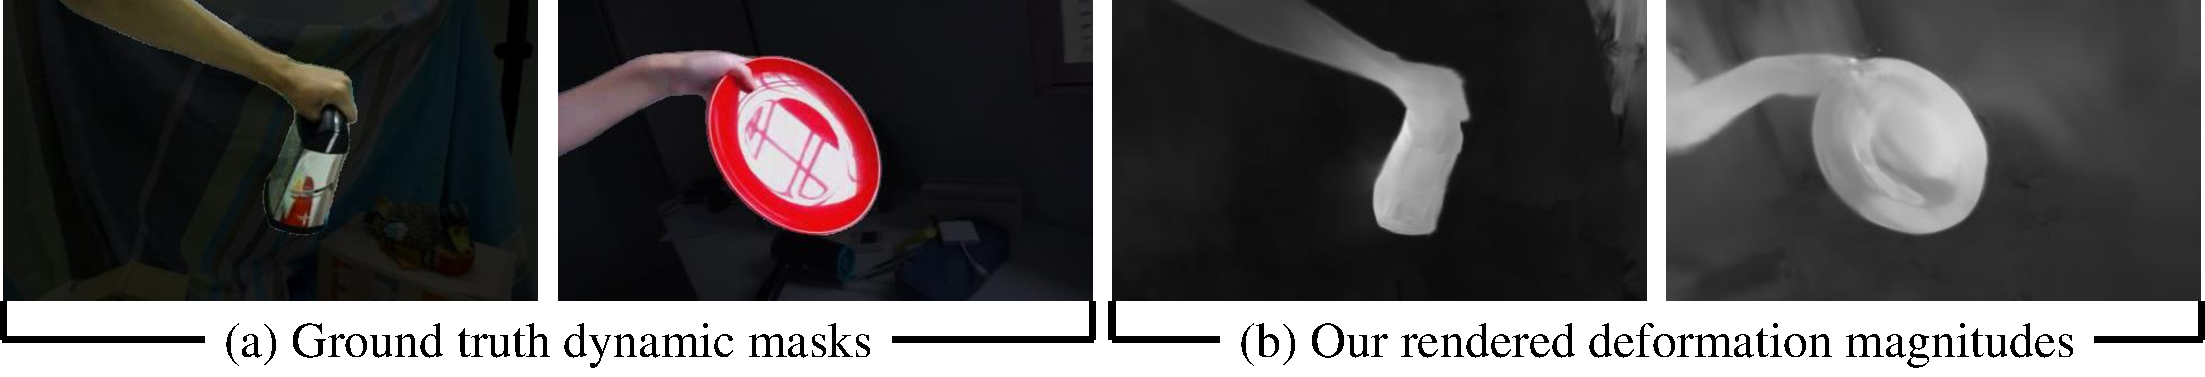
\includegraphics[width=1.0\linewidth]{figures/dynamic_mask.pdf}
    \caption{\textbf{Visualized our deformation magnitudes.} (a) The left side shows the ground truth of the dynamic object, while (b) on the right side, we render the magnitude of the output of the position residual by our deformable Gaussian MLP. The brighter areas indicate greater movement of the 3D Gaussians. The figure shows that even without mask supervision, our method can still effectively distinguish which objects are dynamic.}
    \label{fig:dynamic_mask}
\end{figure*}